%% bare_conf.tex
%% V1.3
%% 2007/01/11
%% by Michael Shell
%% See:
%% http://www.michaelshell.org/
%% for current contact information.
%%
%% This is a skeleton file demonstrating the use of IEEEtran.cls
%% (requires IEEEtran.cls version 1.7 or later) with an IEEE conference paper.
%%
%% Support sites:
%% http://www.michaelshell.org/tex/ieeetran/
%% http://www.ctan.org/tex-archive/macros/latex/contrib/IEEEtran/
%% and
%% http://www.ieee.org/

%%*************************************************************************
%% Legal Notice:
%% This code is offered as-is without any warranty either expressed or
%% implied; without even the implied warranty of MERCHANTABILITY or
%% FITNESS FOR A PARTICULAR PURPOSE! 
%% User assumes all risk.
%% In no event shall IEEE or any contributor to this code be liable for
%% any damages or losses, including, but not limited to, incidental,
%% consequential, or any other damages, resulting from the use or misuse
%% of any information contained here.
%%
%% All comments are the opinions of their respective authors and are not
%% necessarily endorsed by the IEEE.
%%
%% This work is distributed under the LaTeX Project Public License (LPPL)
%% ( http://www.latex-project.org/ ) version 1.3, and may be freely used,
%% distributed and modified. A copy of the LPPL, version 1.3, is included
%% in the base LaTeX documentation of all distributions of LaTeX released
%% 2003/12/01 or later.
%% Retain all contribution notices and credits.
%% ** Modified files should be clearly indicated as such, including  **
%% ** renaming them and changing author support contact information. **
%%
%% File list of work: IEEEtran.cls, IEEEtran_HOWTO.pdf, bare_adv.tex,
%%                    bare_conf.tex, bare_jrnl.tex, bare_jrnl_compsoc.tex
%%*************************************************************************

% *** Authors should verify (and, if needed, correct) their LaTeX system  ***
% *** with the testflow diagnostic prior to trusting their LaTeX platform ***
% *** with production work. IEEE's font choices can trigger bugs that do  ***
% *** not appear when using other class files.                            ***
% The testflow support page is at:
% http://www.michaelshell.org/tex/testflow/



% Note that the a4paper option is mainly intended so that authors in
% countries using A4 can easily print to A4 and see how their papers will
% look in print - the typesetting of the document will not typically be
% affected with changes in paper size (but the bottom and side margins will).
% Use the testflow package mentioned above to verify correct handling of
% both paper sizes by the user's LaTeX system.
%
% Also note that the "draftcls" or "draftclsnofoot", not "draft", option
% should be used if it is desired that the figures are to be displayed in
% draft mode.
%
\documentclass[conference]{IEEEtran}
% Add the compsoc option for Computer Society conferences.
%
% If IEEEtran.cls has not been installed into the LaTeX system files,
% manually specify the path to it like:
% \documentclass[conference]{../sty/IEEEtran}





% Some very useful LaTeX packages include:
% (uncomment the ones you want to load)


% *** MISC UTILITY PACKAGES ***
%
%\usepackage{ifpdf}
% Heiko Oberdiek's ifpdf.sty is very useful if you need conditional
% compilation based on whether the output is pdf or dvi.
% usage:
% \ifpdf
%   % pdf code
% \else
%   % dvi code
% \fi
% The latest version of ifpdf.sty can be obtained from:
% http://www.ctan.org/tex-archive/macros/latex/contrib/oberdiek/
% Also, note that IEEEtran.cls V1.7 and later provides a builtin
% \ifCLASSINFOpdf conditional that works the same way.
% When switching from latex to pdflatex and vice-versa, the compiler may
% have to be run twice to clear warning/error messages.






% *** CITATION PACKAGES ***
%
%\usepackage{cite}
% cite.sty was written by Donald Arseneau
% V1.6 and later of IEEEtran pre-defines the format of the cite.sty package
% \cite{} output to follow that of IEEE. Loading the cite package will
% result in citation numbers being automatically sorted and properly
% "compressed/ranged". e.g., [1], [9], [2], [7], [5], [6] without using
% cite.sty will become [1], [2], [5]--[7], [9] using cite.sty. cite.sty's
% \cite will automatically add leading space, if needed. Use cite.sty's
% noadjust option (cite.sty V3.8 and later) if you want to turn this off.
% cite.sty is already installed on most LaTeX systems. Be sure and use
% version 4.0 (2003-05-27) and later if using hyperref.sty. cite.sty does
% not currently provide for hyperlinked citations.
% The latest version can be obtained at:
% http://www.ctan.org/tex-archive/macros/latex/contrib/cite/
% The documentation is contained in the cite.sty file itself.






% *** GRAPHICS RELATED PACKAGES ***
%
\usepackage{graphicx}
\usepackage{cite}
\usepackage{array}
%\ifCLASSINFOpdf
%  % declare the path(s) where your graphic files are
%  % \graphicspath{{../pdf/}{../jpeg/}}
%  % and their extensions so you won't have to specify these with
%  % every instance of \includegraphics
%  % \DeclareGraphicsExtensions{.pdf,.jpeg,.png}
%\else
%  % or other class option (dvipsone, dvipdf, if not using dvips). graphicx
%  % will default to the driver specified in the system graphics.cfg if no
%  % driver is specified.
%  % \usepackage[dvips]{graphicx}
%  % declare the path(s) where your graphic files are
%  % \graphicspath{{../eps/}}
%  % and their extensions so you won't have to specify these with
%  % every instance of \includegraphics
%  % \DeclareGraphicsExtensions{.eps}
%\fi
% graphicx was written by David Carlisle and Sebastian Rahtz. It is
% required if you want graphics, photos, etc. graphicx.sty is already
% installed on most LaTeX systems. The latest version and documentation can
% be obtained at: 
% http://www.ctan.org/tex-archive/macros/latex/required/graphics/
% Another good source of documentation is "Using Imported Graphics in
% LaTeX2e" by Keith Reckdahl which can be found as epslatex.ps or
% epslatex.pdf at: http://www.ctan.org/tex-archive/info/
%
% latex, and pdflatex in dvi mode, support graphics in encapsulated
% postscript (.eps) format. pdflatex in pdf mode supports graphics
% in .pdf, .jpeg, .png and .mps (metapost) formats. Users should ensure
% that all non-photo figures use a vector format (.eps, .pdf, .mps) and
% not a bitmapped formats (.jpeg, .png). IEEE frowns on bitmapped formats
% which can result in "jaggedy"/blurry rendering of lines and letters as
% well as large increases in file sizes.
%
% You can find documentation about the pdfTeX application at:
% http://www.tug.org/applications/pdftex





% *** MATH PACKAGES ***
%
%\usepackage[cmex10]{amsmath}
% A popular package from the American Mathematical Society that provides
% many useful and powerful commands for dealing with mathematics. If using
% it, be sure to load this package with the cmex10 option to ensure that
% only type 1 fonts will utilized at all point sizes. Without this option,
% it is possible that some math symbols, particularly those within
% footnotes, will be rendered in bitmap form which will result in a
% document that can not be IEEE Xplore compliant!
%
% Also, note that the amsmath package sets \interdisplaylinepenalty to 10000
% thus preventing page breaks from occurring within multiline equations. Use:
%\interdisplaylinepenalty=2500
% after loading amsmath to restore such page breaks as IEEEtran.cls normally
% does. amsmath.sty is already installed on most LaTeX systems. The latest
% version and documentation can be obtained at:
% http://www.ctan.org/tex-archive/macros/latex/required/amslatex/math/





% *** SPECIALIZED LIST PACKAGES ***
%
%\usepackage{algorithmic}
% algorithmic.sty was written by Peter Williams and Rogerio Brito.
% This package provides an algorithmic environment fo describing algorithms.
% You can use the algorithmic environment in-text or within a figure
% environment to provide for a floating algorithm. Do NOT use the algorithm
% floating environment provided by algorithm.sty (by the same authors) or
% algorithm2e.sty (by Christophe Fiorio) as IEEE does not use dedicated
% algorithm float types and packages that provide these will not provide
% correct IEEE style captions. The latest version and documentation of
% algorithmic.sty can be obtained at:
% http://www.ctan.org/tex-archive/macros/latex/contrib/algorithms/
% There is also a support site at:
% http://algorithms.berlios.de/index.html
% Also of interest may be the (relatively newer and more customizable)
% algorithmicx.sty package by Szasz Janos:
% http://www.ctan.org/tex-archive/macros/latex/contrib/algorithmicx/




% *** ALIGNMENT PACKAGES ***
%
%\usepackage{array}
% Frank Mittelbach's and David Carlisle's array.sty patches and improves
% the standard LaTeX2e array and tabular environments to provide better
% appearance and additional user controls. As the default LaTeX2e table
% generation code is lacking to the point of almost being broken with
% respect to the quality of the end results, all users are strongly
% advised to use an enhanced (at the very least that provided by array.sty)
% set of table tools. array.sty is already installed on most systems. The
% latest version and documentation can be obtained at:
% http://www.ctan.org/tex-archive/macros/latex/required/tools/


%\usepackage{mdwmath}
%\usepackage{mdwtab}
% Also highly recommended is Mark Wooding's extremely powerful MDW tools,
% especially mdwmath.sty and mdwtab.sty which are used to format equations
% and tables, respectively. The MDWtools set is already installed on most
% LaTeX systems. The lastest version and documentation is available at:
% http://www.ctan.org/tex-archive/macros/latex/contrib/mdwtools/


% IEEEtran contains the IEEEeqnarray family of commands that can be used to
% generate multiline equations as well as matrices, tables, etc., of high
% quality.


%\usepackage{eqparbox}
% Also of notable interest is Scott Pakin's eqparbox package for creating
% (automatically sized) equal width boxes - aka "natural width parboxes".
% Available at:
% http://www.ctan.org/tex-archive/macros/latex/contrib/eqparbox/





% *** SUBFIGURE PACKAGES ***
%\usepackage[tight,footnotesize]{subfigure}
% subfigure.sty was written by Steven Douglas Cochran. This package makes it
% easy to put subfigures in your figures. e.g., "Figure 1a and 1b". For IEEE
% work, it is a good idea to load it with the tight package option to reduce
% the amount of white space around the subfigures. subfigure.sty is already
% installed on most LaTeX systems. The latest version and documentation can
% be obtained at:
% http://www.ctan.org/tex-archive/obsolete/macros/latex/contrib/subfigure/
% subfigure.sty has been superceeded by subfig.sty.



%\usepackage[caption=false]{caption}
%\usepackage[font=footnotesize]{subfig}
% subfig.sty, also written by Steven Douglas Cochran, is the modern
% replacement for subfigure.sty. However, subfig.sty requires and
% automatically loads Axel Sommerfeldt's caption.sty which will override
% IEEEtran.cls handling of captions and this will result in nonIEEE style
% figure/table captions. To prevent this problem, be sure and preload
% caption.sty with its "caption=false" package option. This is will preserve
% IEEEtran.cls handing of captions. Version 1.3 (2005/06/28) and later 
% (recommended due to many improvements over 1.2) of subfig.sty supports
% the caption=false option directly:
%\usepackage[caption=false,font=footnotesize]{subfig}
%
% The latest version and documentation can be obtained at:
% http://www.ctan.org/tex-archive/macros/latex/contrib/subfig/
% The latest version and documentation of caption.sty can be obtained at:
% http://www.ctan.org/tex-archive/macros/latex/contrib/caption/




% *** FLOAT PACKAGES ***
%
%\usepackage{fixltx2e}
% fixltx2e, the successor to the earlier fix2col.sty, was written by
% Frank Mittelbach and David Carlisle. This package corrects a few problems
% in the LaTeX2e kernel, the most notable of which is that in current
% LaTeX2e releases, the ordering of single and double column floats is not
% guaranteed to be preserved. Thus, an unpatched LaTeX2e can allow a
% single column figure to be placed prior to an earlier double column
% figure. The latest version and documentation can be found at:
% http://www.ctan.org/tex-archive/macros/latex/base/



%\usepackage{stfloats}
% stfloats.sty was written by Sigitas Tolusis. This package gives LaTeX2e
% the ability to do double column floats at the bottom of the page as well
% as the top. (e.g., "\begin{figure*}[!b]" is not normally possible in
% LaTeX2e). It also provides a command:
%\fnbelowfloat
% to enable the placement of footnotes below bottom floats (the standard
% LaTeX2e kernel puts them above bottom floats). This is an invasive package
% which rewrites many portions of the LaTeX2e float routines. It may not work
% with other packages that modify the LaTeX2e float routines. The latest
% version and documentation can be obtained at:
% http://www.ctan.org/tex-archive/macros/latex/contrib/sttools/
% Documentation is contained in the stfloats.sty comments as well as in the
% presfull.pdf file. Do not use the stfloats baselinefloat ability as IEEE
% does not allow \baselineskip to stretch. Authors submitting work to the
% IEEE should note that IEEE rarely uses double column equations and
% that authors should try to avoid such use. Do not be tempted to use the
% cuted.sty or midfloat.sty packages (also by Sigitas Tolusis) as IEEE does
% not format its papers in such ways.





% *** PDF, URL AND HYPERLINK PACKAGES ***
%
%\usepackage{url}
% url.sty was written by Donald Arseneau. It provides better support for
% handling and breaking URLs. url.sty is already installed on most LaTeX
% systems. The latest version can be obtained at:
% http://www.ctan.org/tex-archive/macros/latex/contrib/misc/
% Read the url.sty source comments for usage information. Basically,
% \url{my_url_here}.





% *** Do not adjust lengths that control margins, column widths, etc. ***
% *** Do not use packages that alter fonts (such as pslatex).         ***
% There should be no need to do such things with IEEEtran.cls V1.6 and later.
% (Unless specifically asked to do so by the journal or conference you plan
% to submit to, of course. )


% correct bad hyphenation here
%\hyphenation{op-tical net-works semi-conduc-tor}

\newtheorem{definition}{Definition}
\newtheorem{proposition}{Proposition}

\begin{document}
%
% paper title
% can use linebreaks \\ within to get better formatting as desired
\title{A Hardware Architecture for Filtering Irreducible Testors}


% author names and affiliations
% use a multiple column layout for up to three different
% affiliations
%\author{\IEEEauthorblockN{Vlad\'imir Rodr\'iguez Diez}
%\IEEEauthorblockA{Electrical Engineering School\\
%University of Camaguey\\
%Camaguey, Cuba\\
%Email: vladimir.rodriguez@reduc.edu.cu}
%\and
%\IEEEauthorblockN{Jos\'e F. Mart\'inez,
%				 Jes\'us A. Carrasco\\
%				 Manuel S. Lazo,
%				 Ren\'e A. Cumplido\\
%				 and Claudia Feregrino}
%\IEEEauthorblockA{Computer Science Department\\
%				National Institute for Astrophysics, Optics and Electronics\\
%				Sta. Ma. Tonanzintla, Puebla, 72840, Mexico}}
%Email: homer@thesimpsons.com}
%\and
%\IEEEauthorblockN{James Kirk\\ and Montgomery Scott}
%\IEEEauthorblockA{Starfleet Academy\\
%San Francisco, California 96678-2391\\
%Telephone: (800) 555--1212\\
%Fax: (888) 555--1212}}

% conference papers do not typically use \thanks and this command
% is locked out in conference mode. If really needed, such as for
% the acknowledgment of grants, issue a \IEEEoverridecommandlockouts
% after \documentclass

% for over three affiliations, or if they all won't fit within the width
% of the page, use this alternative format:
% 
\author{aa}




% use for special paper notices
%\IEEEspecialpapernotice{(Invited Paper)}




% make the title area
\maketitle


\begin{abstract}
	Feature selection is an important task in pattern recognition. Given a dataset described by a set of attributes, a minimum subset of attributes that preserves the ability to discern between objects from different classes is needed. The computation of this minimum subset is a problem whose space complexity grows
exponentially regarding the number of attributes. Testor Theory is a convenient way to solve this problem. A testor is defined as a subset of attributes that can discern between objects of different classes; and an irreducible testor is a minimal subset with this property. There are several hardware implementations of algorithms for computing testors; which take advantage of the inherent parallelism in the evaluation of testor candidates. In this paper, a new hardware module for filtering irreducible testors from computed testors set is presented.
\end{abstract}
% IEEEtran.cls defaults to using nonbold math in the Abstract.
% This preserves the distinction between vectors and scalars. However,
% if the conference you are submitting to favors bold math in the abstract,
% then you can use LaTeX's standard command \boldmath at the very start
% of the abstract to achieve this. Many IEEE journals/conferences frown on
% math in the abstract anyway.

% no keywords




% For peer review papers, you can put extra information on the cover
% page as needed:
% \ifCLASSOPTIONpeerreview
% \begin{center} \bfseries EDICS Category: 3-BBND \end{center}
% \fi
%
% For peerreview papers, this IEEEtran command inserts a page break and
% creates the second title. It will be ignored for other modes.
\IEEEpeerreviewmaketitle



\section{Introduction}
Nowadays, the feature selection problem in pattern recognition is usually characterized by a large number of 
attributes. The feature selection process consists in identifying those attributes that provide relevant 
information for the classification process. 
Testor Theory is an effective way to deal with feature selection.
% as shownin~\cite{Ruiz08, Martinez01}. 
 A testor is defined as a subset of attributes capable of discerning objects from 
different classes. An irreducible testor is a testor such that every attribute is indispensable for satisfying 
the testor condition. The problem of finding all irreducible testors has been proven NP-hard~\cite{Skowron92}.

Reconfigurable computing using Field Programmable Gate-Array (FPGA) has become a powerful alternative to handle 
complex computational problems. 
%Recently, several hardware-software platforms using FPGA have been reported~ \cite{Compton02,Pocek13}. 
Hardware-software platforms take advantage of custom design to perform those operations with a high
parallelism degree on the FPGA device, while complementary tasks are executed by a software component in a PC.

The first implementation of Testor Theory algorithms on FPGA~\cite{Cumplido06} was a brute force approach for 
computing testors. In this first approach all the $2^n$ combinations of $n$ attributes are tested in order to 
select only those which are testors. Afterwards, in \cite{Rojas07} a hardware implementation of the Bottom-Top 
(BT) algorithm for computing irreducible testors was introduced. 
The BT algorithm uses a candidate pruning process for avoiding unnecessary candidate evaluation, 
reducing this way the number of iterations needed. These two previous platforms computed a set of testors on the 
FPGA device whilst irreducible condition was evaluated afterwards by the software component in a hosting PC. 
In \cite{Rojas12} a hardware-software platform for computing irreducible testors implementing the BT algorithm, 
as in \cite{Rojas07}, was presented. This last architecture also included a new module that eliminates most of 
the non irreducible testors before transferring them to a host software application for final filtering. 

Main disadvantages of these approaches are the huge amount of data that must be transferred to the PC and the 
extra cost of the final filtering stage in the software component.  
For this reason, in this paper, we develop a hardware module for eliminating all non irreducible testors 
on the FPGA device, reducing the amount of data that must be transferred to the PC. This architecture is 
applicable to any algorithm for computing irreducible testors implemented in FPGA, since it operates in the 
candidate evaluation process.

The rest of this paper is structured as follows. Section~\ref{sect:2} introduces the basic concepts of 
Testor Theory. Section~\ref{sect:3} introduces the proposed architecture. Evaluation of the proposed 
architecture and a discussion of the experimental results are presented in section~\ref{sect:6}. Finally,
section~\ref{sect:8} shows our conclusions.

\section{Basic concepts}
\label{sect:2}

In pattern recognition, feature selection is a very important task for Supervised Classification. In the logical
 combinatorial approach to pattern recognition \cite{Martinez01}, a useful
way to deal with this problem is through Testor Theory. The concept of testor for pattern recognition was
introduced by \cite{Dmitriev66}. They defined a testor as a subset of features that allows
differentiating objects from different classes. Testors are quite useful, especially when object descriptions
contain both numeric and non-numeric features, and maybe they are incomplete (mixed incomplete data)
\cite{Martinez01}. 
%This concept has been developed in different contexts \cite{Lazo01}. From an 
%algorithmic point of view, Testor Theory has shown a continuous development from its origins to the present 
%\cite{Ruiz85,Sanchez02,Sanchez10}.

Let $TM$ be a training matrix with $k$ objects described through $n$
features of any type $\{x_{1},\ldots,x_{n}\}$ and grouped in $r$
classes. Let $DM$ be a Boolean dissimilarity matrix (0 = similar, 1 =
dissimilar), obtained from a feature by feature comparison of every
pair of objects from $TM$ belonging to different classes. $DM$ has
$m$ rows and $n$ columns, where usually $m>>k$.

Let $T$ be a subset of attributes. Testors and irreducible testors are formally defined as follows:

\begin{definition} \label{def1}
$T$ is a testor if and only if when all
features (columns) are eliminated from $DM$, except those from $T$, there is
not any row of $DM$ with only 0's. $T$ is an irreducible testor if none of its proper subsets is a testor.
\end{definition}

In defintion \ref{def1}, if there is not any row of $DM$ with only
0's it means that there is not a pair of objects from different
classes that are similar on all the features of $T$, that is, a
testor $T$ allows differentiating objects from different
classes. From definition~\ref{def1}, if $T$ is a testor then, any superset of $T$ is a testor too.

The number of rows in $DM$ could be too large, therefore a strategy to reduce this matrix, without losing
relevant information for computing irreducible testors, is eliminating redundant rows \cite{Lazo01}.

%% DEFINICION 
\begin{definition}
Let $f=[f_1, f_2, \dots , f_n]$ and $f'=[f'_1, {f'}_2, \dots , {f'}_n]$ be two rows of $DM$, $f$ 
is a sub-row of $f^{'}$ if for each column $j=1,2,\dots ,n$;  $f_{j} \le f'_{j}$ and for at least one index, the 
inequality is strict.
\end{definition}

%% DEFINICION 
\begin{definition}
A row $f$ of $DM$ is a basic row if no row of the matrix $DM$ is a sub-row of $f$. 
\end{definition}

%% DEFINICION 
\begin{definition}
The basic matrix of $DM$, denoted as $BM$, is the sub-matrix of $DM$ formed only by the basic rows (without 
repetitions).

\end{definition}

Let $TT(DM)$ and $TT(BM)$ be the sets of all irreducible testors of $DM$ and $BM$ respectively, it is 
relatively easy to prove that $TT(DM)=TT(BM)$, see \cite{Lazo95}; i.e., we can conclude that usually $DM$ 
contains redundant information. In addition, the construction of $BM$ from $DM$ is a very fast process, 
then we work over $BM$.

%The CT-EXT algorithm has the following theoretical bases.

\begin{definition} \label{def21} Let $f_i$ be a row of BM, $f_i$ is a zero row of $S \subseteq R$, and we denote it as ${f_i}^0 (S)$, if $\forall x_p \in S$, $f_i [p] = BM [i, p] = 0$. We denote as $\Sigma_S f^0$  the amount of zero rows of S.
\end{definition}
\begin{definition} \label{def22} In terms of BM, a testor $T \subseteq R$ is a feature set such that there
are no zero rows of T in BM. 
\end{definition}
\begin{definition} \label{def23} Let $f_i$ be a row of BM, $f_i$ is a typical row of $S \subseteq R$ regarding $x_q$, being $x_q \in S$, and we denote it by ${f_i}^1 (S,q)$ if $f_i [q] = BM [i, q] = 1$, and $\forall x_p \in S$, $x_p \neq x_q$ , $f_i [p] = BM [i, p] =~0$.
\end{definition}

\begin{definition} \label{def24} In terms of BM, $T \subseteq R$ is an irreducible testor if T is a testor and
$\forall x_j \in T, \exists {f_i}^1 (T, j)$.
\end{definition}

This means that for each feature in an irreducible testor, there exists a row in 
the sub matrix of $BM$ associated to $T$, having a 1 in the position corresponding
to that feature, and 0 in all remaining positions (if any column of $T$ is eliminated, 
at least one zero row will appear, and the testor property would not be fulfilled). 

\section{Proposed architecture}
\label{sect:3}

Computing all irreducible testors has exponential complexity regarding the number of attributes. Each 
algorithm for irreducible testors computation has its own strategy for traversing the search space 
consisting of the $2^n$ combinations of $n$ attributes; nevertheless, no matter the strategy used,
a necessary stage for all these algorithms is the verification of each candidate combination 
over the basic matrix to fulfill definition~\ref{def22}. Hardware implementations have a common module 
holding the basic matrix data, which is responsible for this verification. Our proposed architecture consists in 
modifying this module which can be ported to any algorithm implementation. We will introduce the 
new architecture in the top of the platform presented in~\cite{Rojas12}.

In the hardware platform, a feature subset is handled as an $n$-tuple, using a positional 
representation for all the $n$ attributes of a basic matrix $BM$. Given a subset $T$, its $n$-tuple 
representation has a 1 in the corresponding position $j$ for each $x_j \in T$ and 0 otherwise.
Fig.\,\ref{figOldArq} shows the original platform for testors computation as in \cite{Rojas12}. This 
architecture consists of three main modules: the \textit{Candidate Generator}, the $BM$ and the 
\textit{Dismiss Testors}.

The \textit{Candidate Generator} module handles the sequence of candidates to be evaluated. In order to 
calculate the next candidate, this module receives some feedback information from the $BM$ module. The 
\textit{Candidate Generator} module is specific and its internal design is beyond the goal of this paper.
The $BM$ module handles the process of deciding whether an $n$-tuple is a testor of $BM$,
comparing the candidate against each one of the $BM$'s rows. Since our modifications take place in this 
module, we will expose it in detail afterwards. Finally, the \textit{Dismiss Testors} module filters most 
non irreducible testors by checking inclusion of every new testor in each register of an output FIFO \cite{Rojas12}.

\begin{figure}[htb]
    \centering
    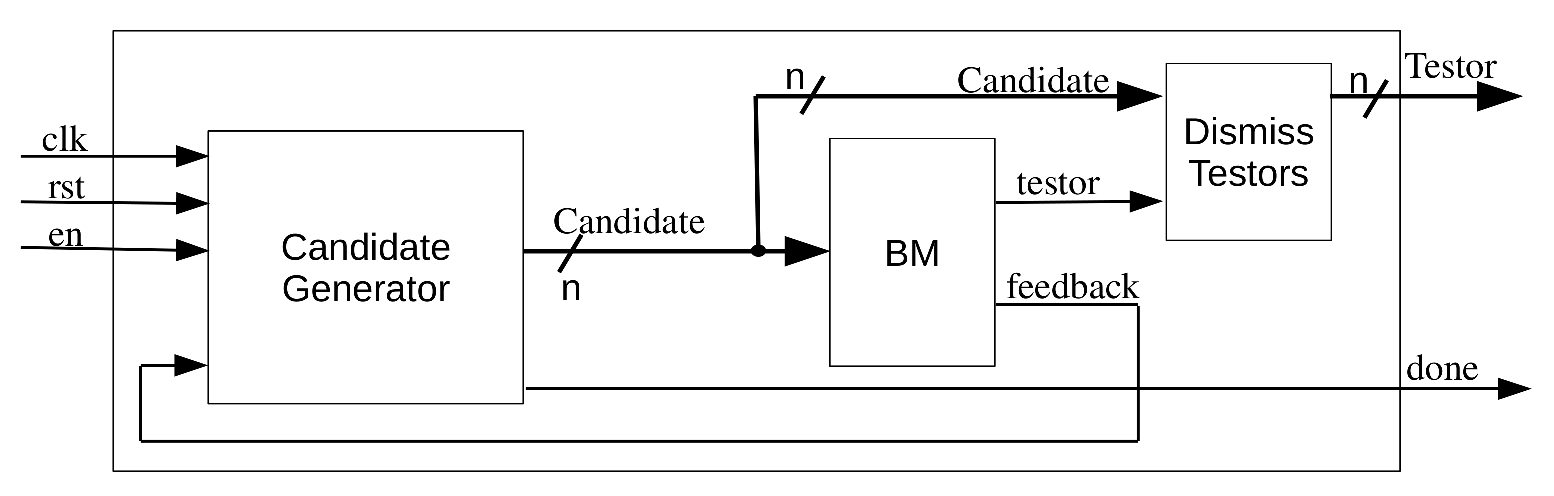
\includegraphics[width=7cm]{old_arq.eps}
	\caption{Previous Architecture.}
	\label{figOldArq}
\end{figure}

The modified architecture for finding irreducible testors is shown in Fig.\,\ref{figNewArq}. It can be seen 
that the \textit{Dismiss Testors} module is no longer needed since we have a signal indicating whether the 
current candidate is an irreducible testor or not. 

\begin{figure}[htb]
    \centering
    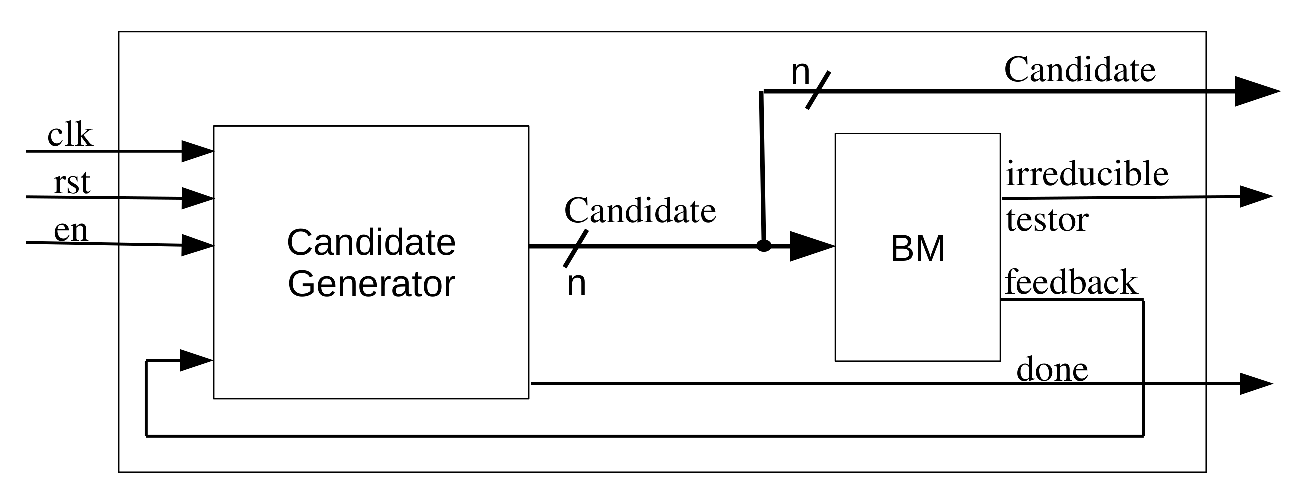
\includegraphics[width=7cm]{new_arq.eps}
	\caption{Proposed Architecture.}
	\label{figNewArq}
\end{figure}



\begin{figure}[htb]
    \centering
    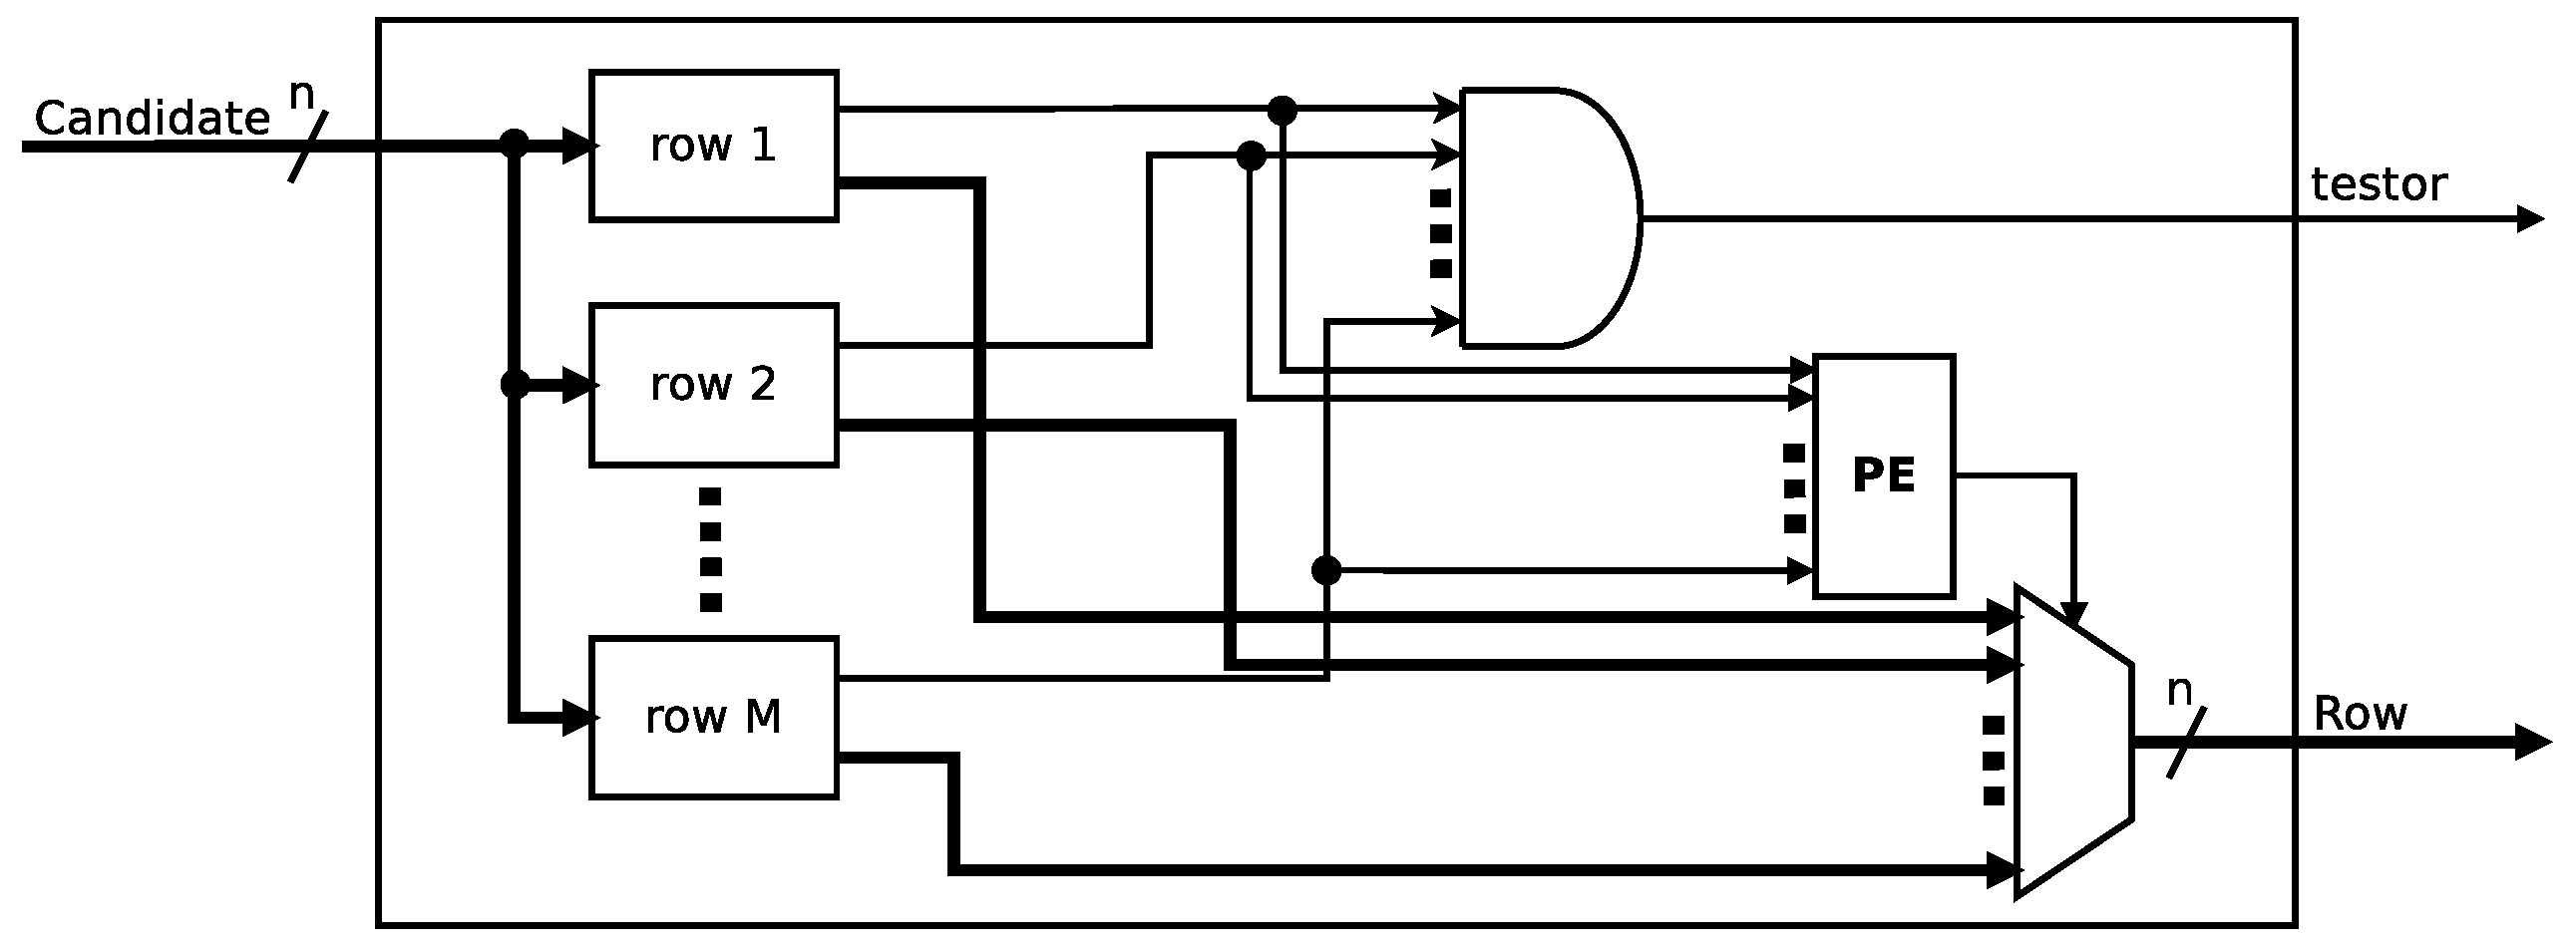
\includegraphics[width=7cm]{BM_module_old.eps}
	\caption{Original $BM$ module.}
	\label{figBMold}
\end{figure}

The original $BM$ module is composed of $M$ sub-modules named \textit{row~i}, as shown
in Fig.\,\ref{figBMold}. Each \textit{row~i} module contains a row ($n$ bits)
of the basic matrix and the logic needed to perform testor evaluation. To decide
whether an $n$-tuple is a testor, a bitwise AND operation is performed
between the constant stored in each \textit{row~i} module and the current
candidate, as shown in Fig.\,\ref{figBMrowOld}. If at least one bit of the AND operation is TRUE,
then the output \textit{testor} of that particular \textit{row~i} sub-module is also TRUE. 
If the output $testor$ of all  \textit{row~i} sub-modules is
TRUE, then the output \textit{testor} of the $BM$ module is TRUE,
which means that the candidate is a testor of $BM$.
A priority encoder is used to select the $n$-tuple holding the data corresponding to the upper row 
of $BM$ which does not satisfy the testor condition. This information is used by the \textit{Candidate Generator}
module given that the current candidate is not a testor \cite{Rojas12}.

\begin{figure}[htb]
\centering
\begin{minipage}{4cm}
  \centering
   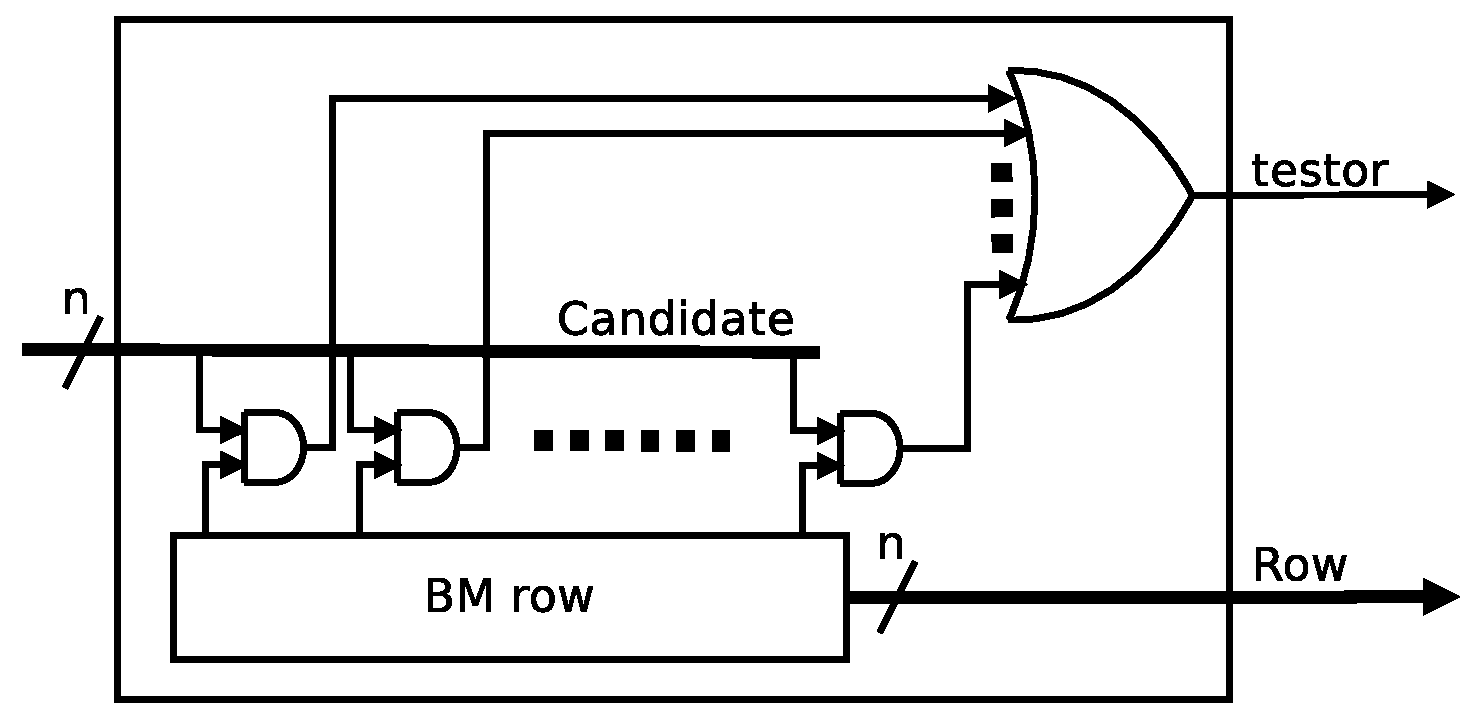
\includegraphics[width=4cm]{BM_row_old.eps}
	\caption{Original $BM$ row.}
	\label{figBMrowOld}
\end{minipage}%
\begin{minipage}{4.8cm}
  \centering
  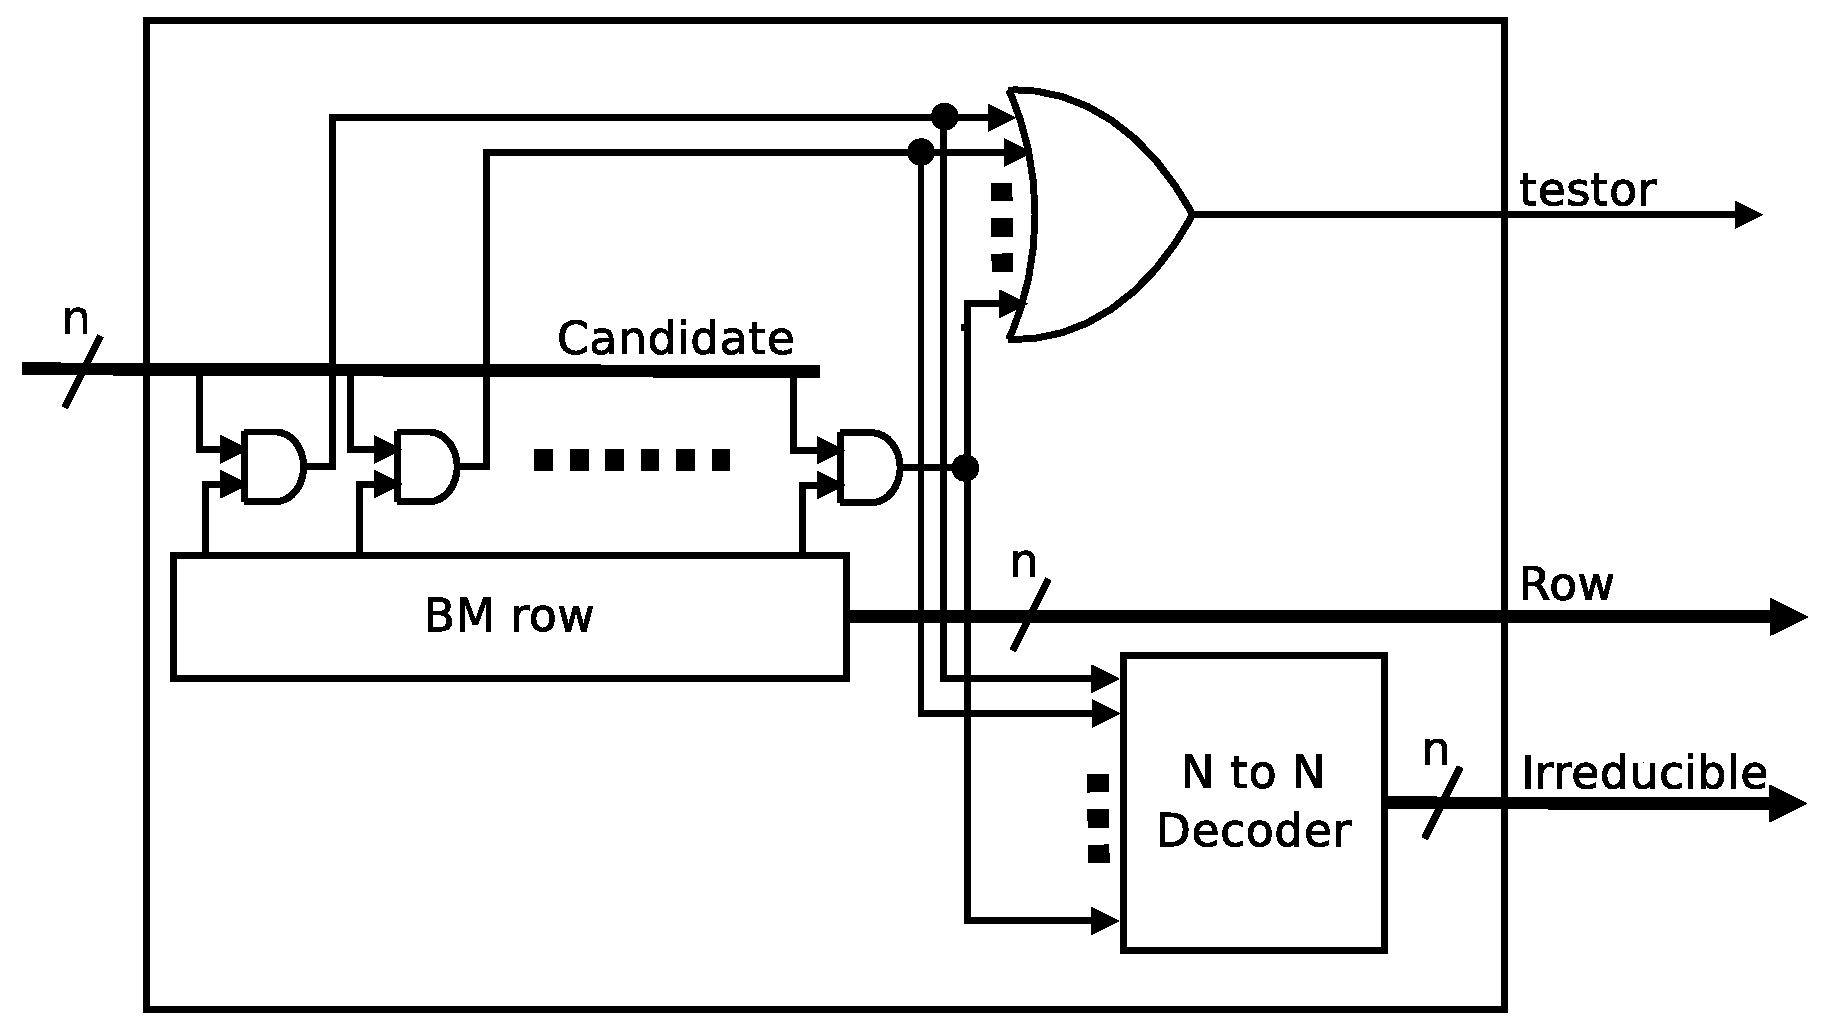
\includegraphics[width=4.8cm]{BM_row_new.eps}
	\caption{Proposed $BM$ row.}
	\label{figBMrowNew}
\end{minipage}
\end{figure}

%\begin{figure}[htb]
%    \centering
%    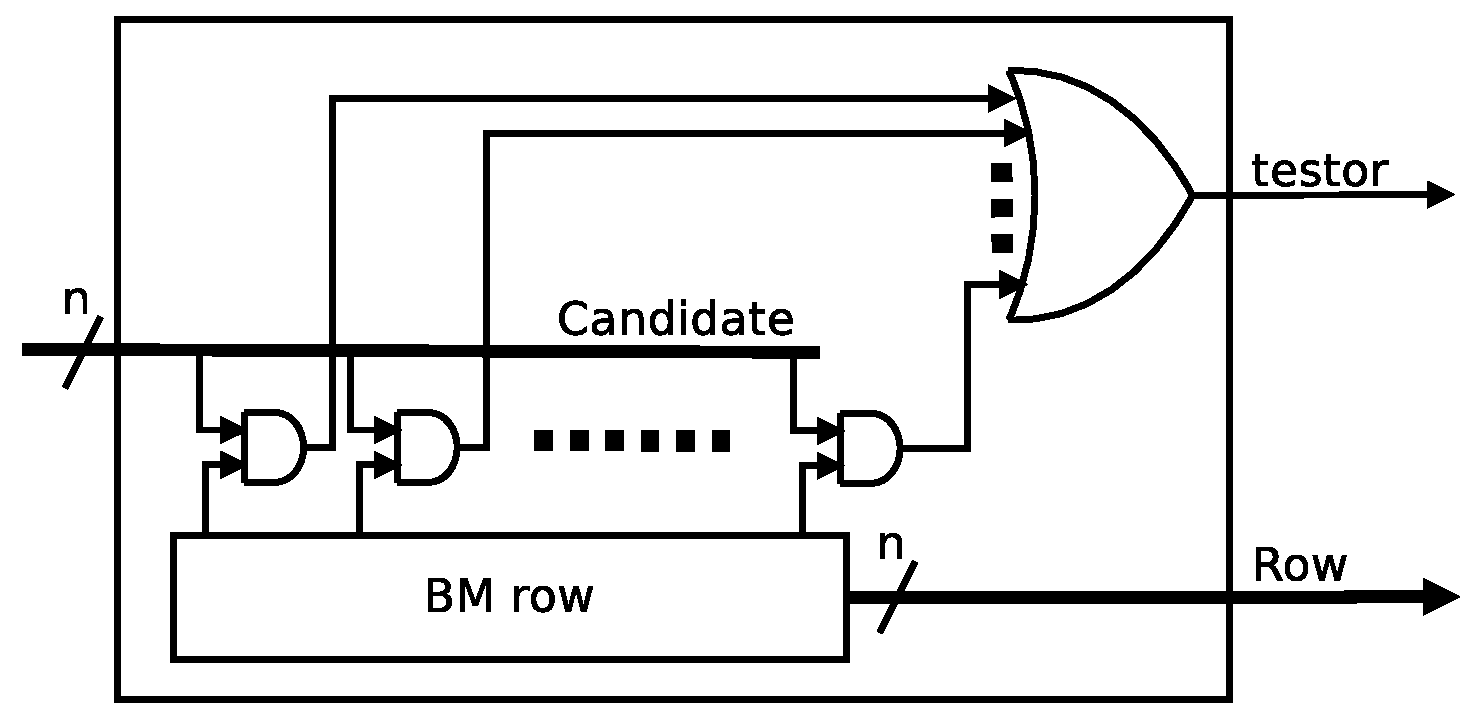
\includegraphics[width=5cm]{BM_row_old.eps}
%	\caption{Original $BM$ row.}
%	\label{figBMrowOld}
%\end{figure}
%
%\begin{figure}[htb]
%    \centering
%    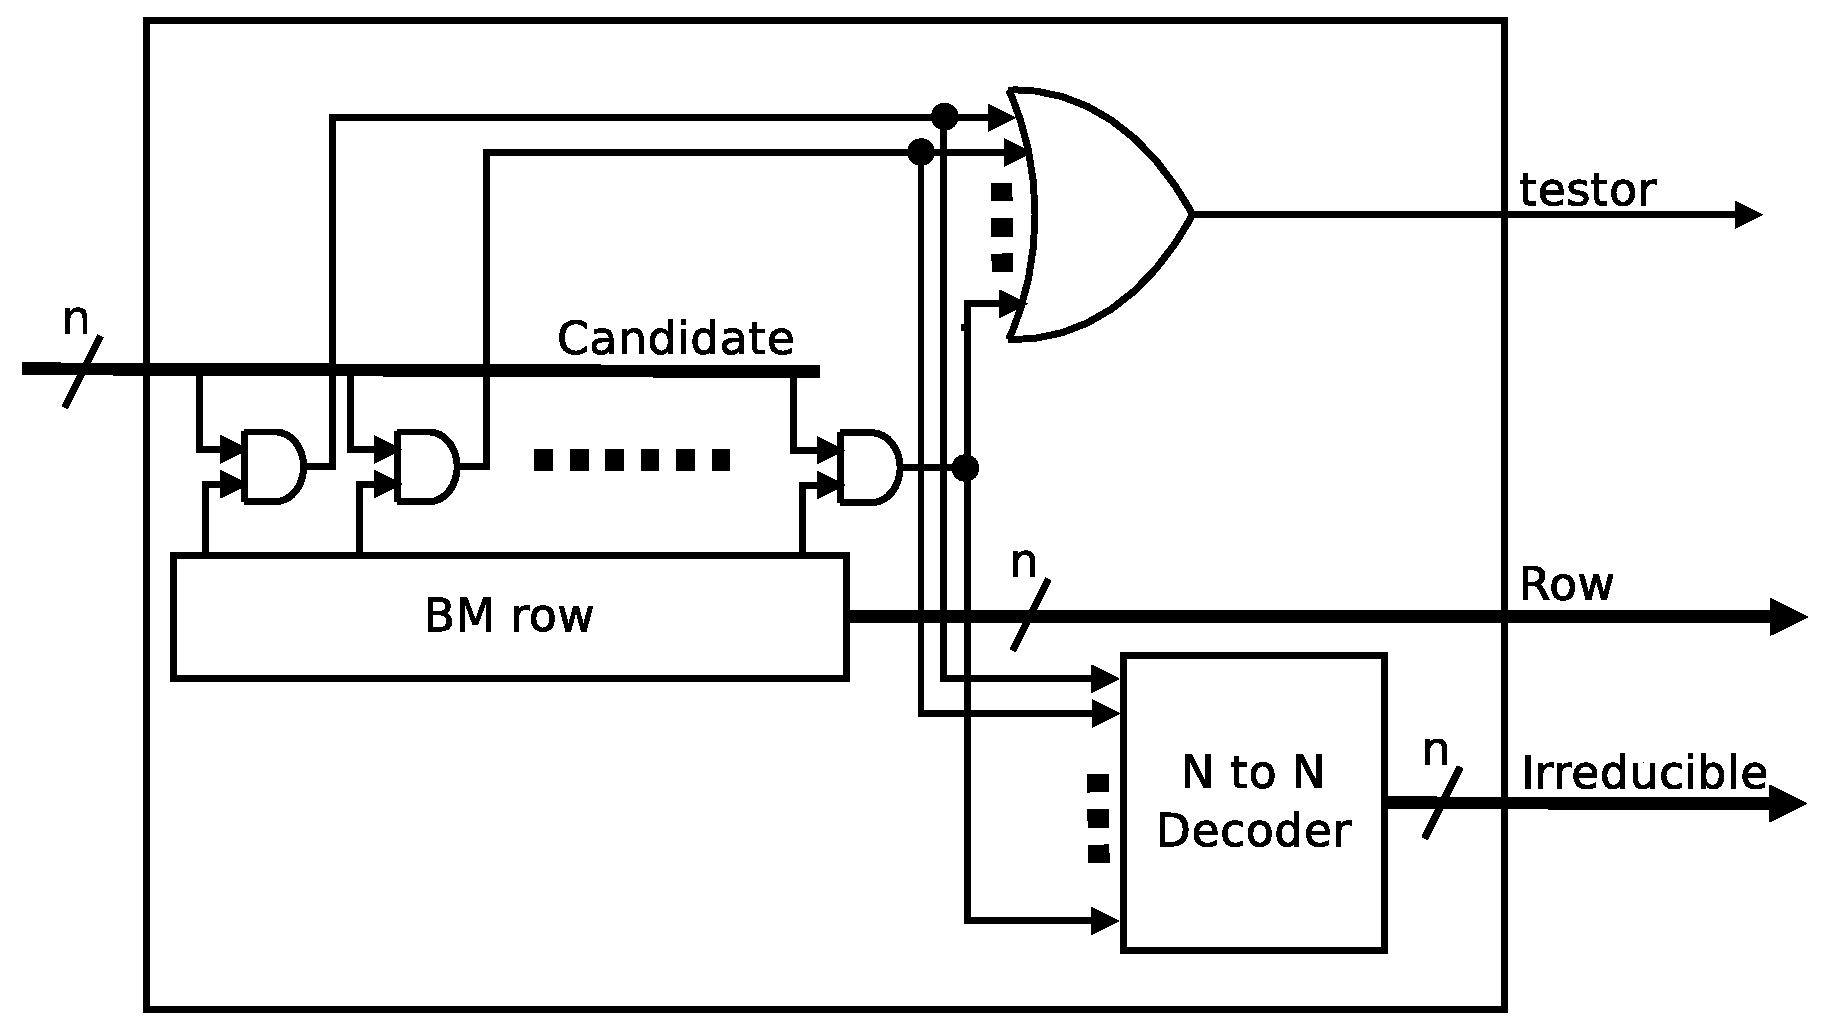
\includegraphics[width=5cm]{BM_row_new.eps}
%	\caption{Proposed $BM$ row.}
%	\label{figBMrowNew}
%\end{figure}

In our proposed architecture, an \textit{N~to~N~Decoder} is introduced into each 
\textit{row~i} module, as shown in Fig.\,\ref{figBMrowNew}. This new component receives as input 
the result of the AND operation between the current candidate and the corresponding $BM$ row.
The output from the \textit{N~to~N~Decoder} repeats the input when there is only one bit set
to 1, and returns the null $n$-tuple $(0,...,0)$ otherwise. For those rows with only one bit having a 1 after ANDed with the candidate, the attribute in the position of that bit is indispensable if the candidate is a testor.

According to definition~\ref{def24}, every attribute in a testor must be indispensable to be an
irreducible testor. Fig.\,\ref{figBMnew} shows the modified $BM$ module for the evaluation of 
irreducible testors. Two operations are added to this module in order to verify the condition stated in 
definition~\ref{def24}. First, a bitwise OR operation is performed among the output $Irreducible$ of all 
\textit{row~i} submodules. The result of this operation has a 1 in the positions corresponding to each 
indispensable attribute in the current candidate. This value is then compared to the current candidate, 
and the output \textit{irreducible testor} is TRUE given that this comparison holds equality and 
the output $testor$ of the $BM$ module is TRUE.

\begin{figure}[htb]
    \centering
	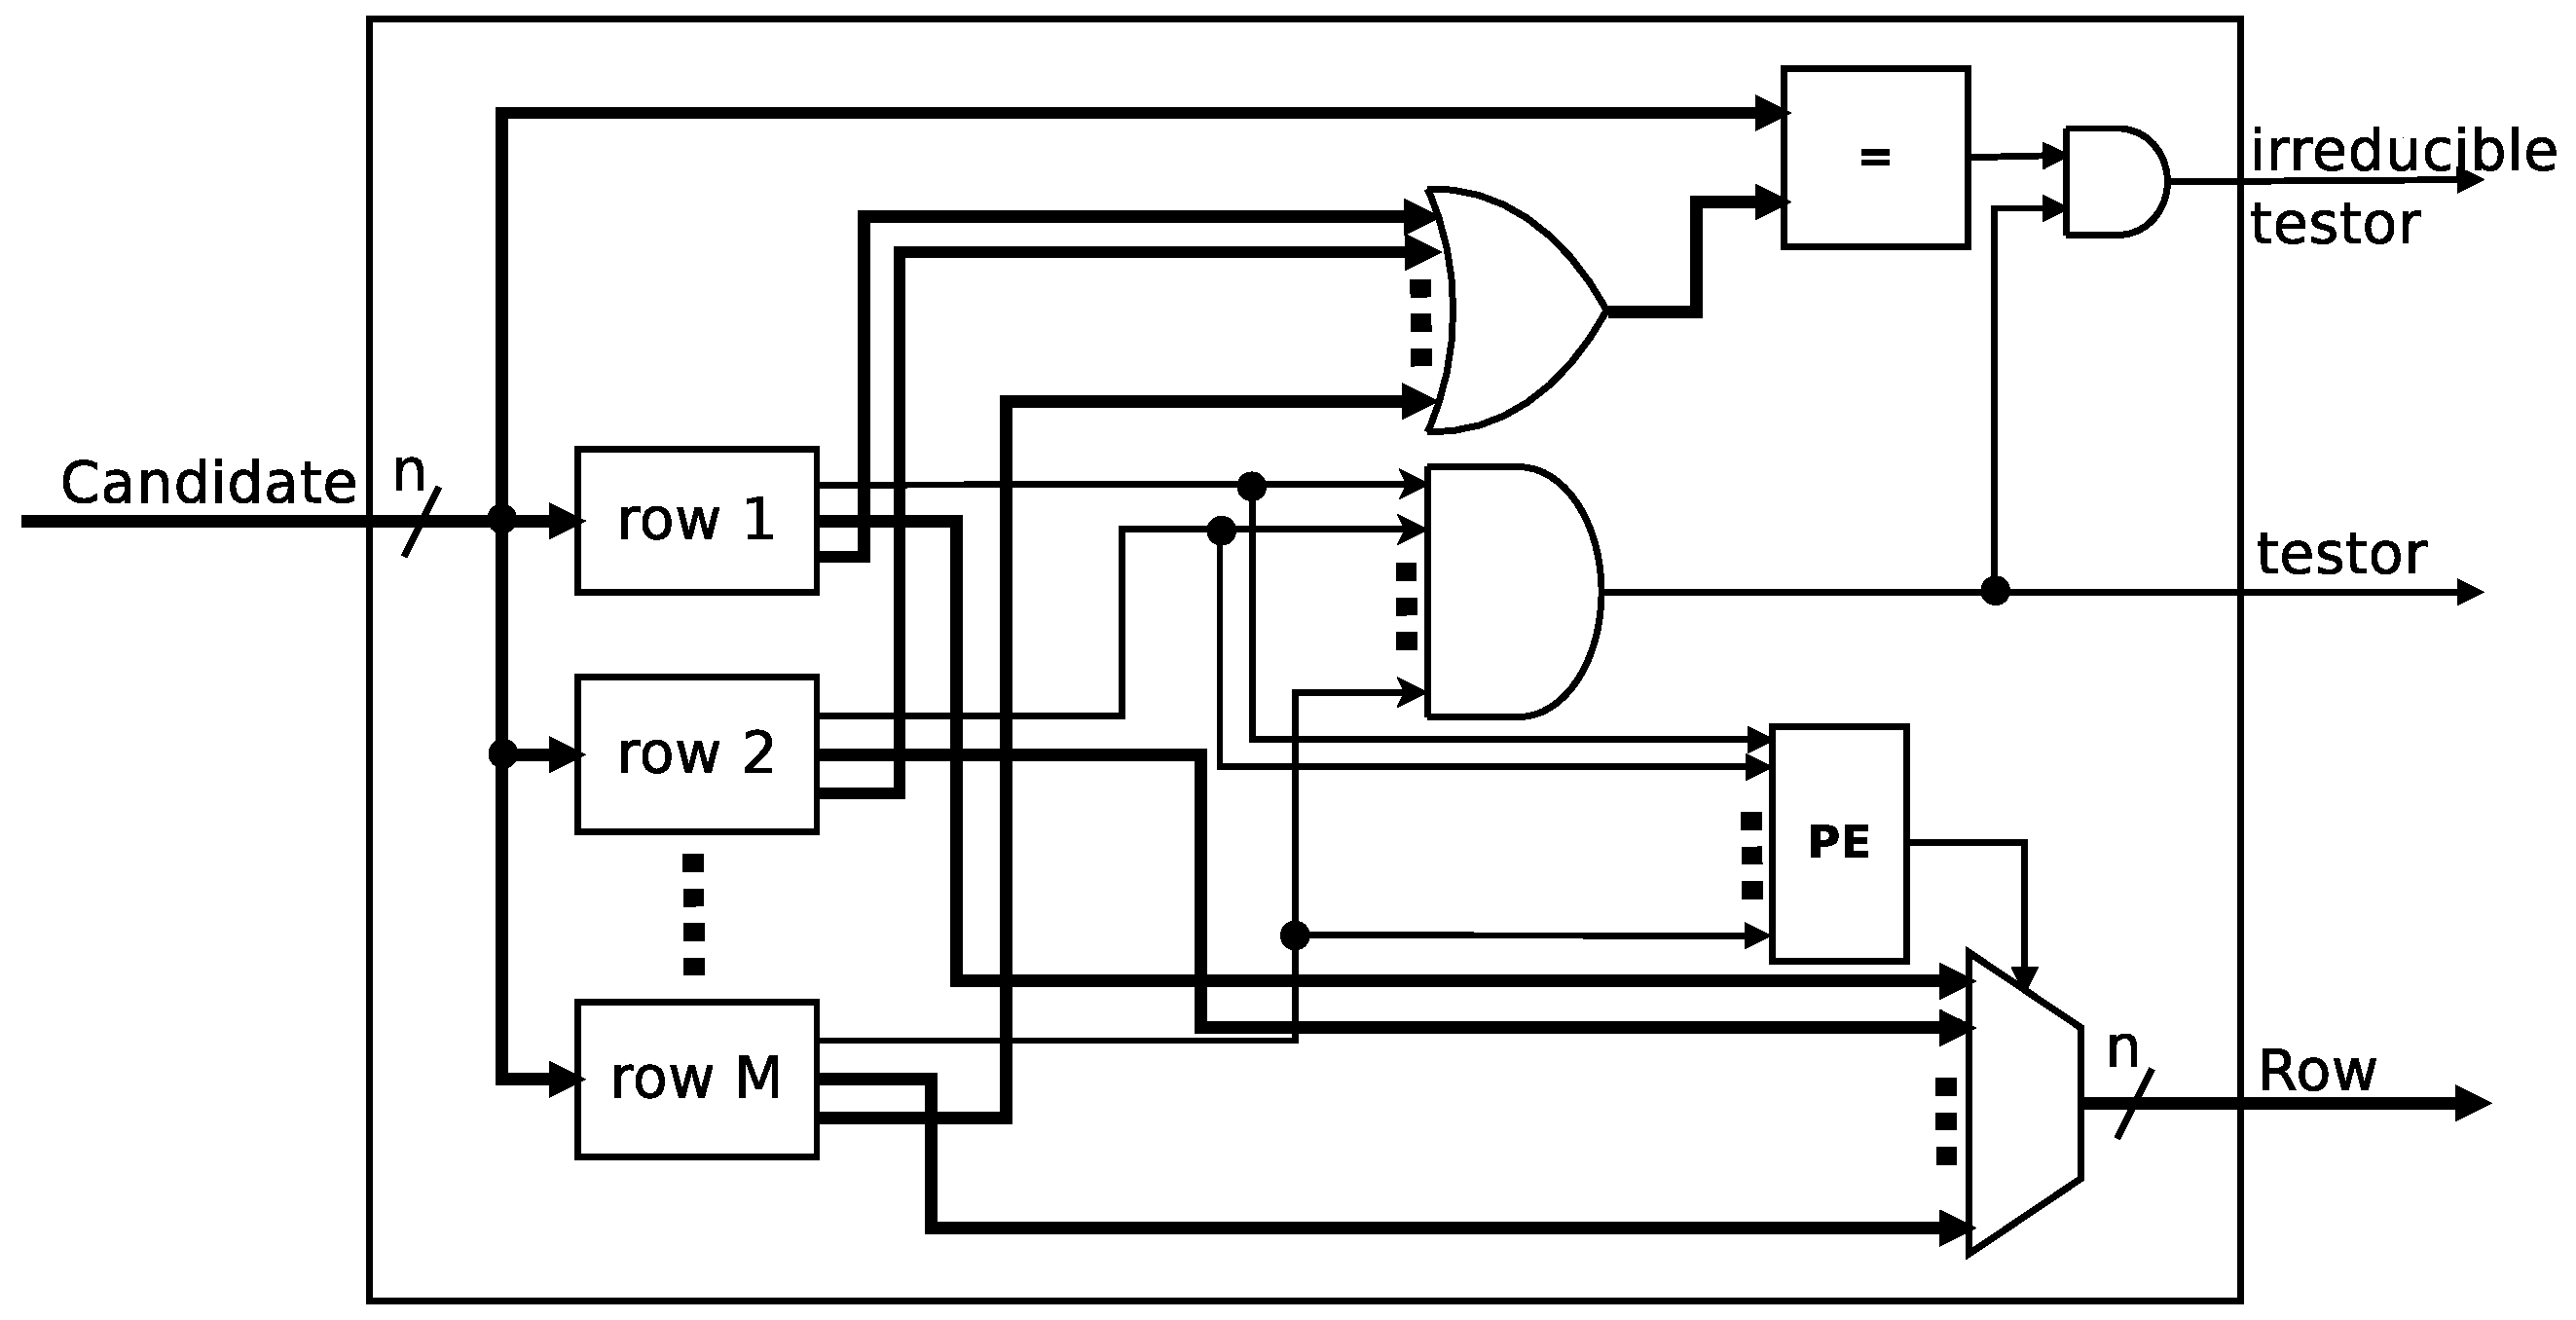
\includegraphics[width=7cm]{BM_module_new.eps}
	\caption{Proposed $BM$ module.}
	\label{figBMnew}
\end{figure}

\begin{table}[htb]
	\renewcommand{\arraystretch}{1.3}
	\caption{Basic matrix}
	\label{tabBM}
	\centering
	\begin{tabular}{cccc}
	 	\hline                       
	  	$x_0$ & $x_1$ & $x_2$ & $x_3$\\
	  	\hline
	  	1 & 1 & 0 & 0 \\
	  	1 & 0 & 1 & 0 \\
	  	0 & 1 & 0 & 1 \\
	 	\hline 
	\end{tabular}
\end{table}

Lets us take for example the basic matrix shown in Table~\ref{tabBM}. We are going to illustrate the 
operation of the proposed architecture using two testors for this basic matrix. First we will evaluate 
the candidate $\{x_0,x_1\}$ which is an irreducible testor. Secondly, the candidate $\{x_0,x_1,x_2\}$ will 
be evaluated. This last attribute set is a superset of $\{x_0,x_1\}$ and thus, it is not an irreducible testor.


\begin{table}[htb]
	\renewcommand{\arraystretch}{1.3}
	\caption{An example of irreducible testor}
	\label{tabIrreducible}
	\centering
	\begin{tabular}{cccc|cccc}
	 	\hline                       
  		\multicolumn{4}{c|}{Cand. $\{x_0, x_1\}$} & 
  		\multicolumn{4}{c}{Decoder output} \\
  		\hline
		$x_0$ & $x_1$ & $x_2$ & $x_3$ &
  		$x_0$ & $x_1$ & $x_2$ & $x_3$\\
  		\hline
  		1 & 1 & 0 & 0 & 0 & 0 & 0 & 0\\
  		1 & 0 & 0 & 0 & 1 & 0 & 0 & 0\\
  		0 & 1 & 0 & 0 & 0 & 1 & 0 & 0\\
  		\hline  
  		\multicolumn{4}{c|}{Candidate $=$} & 1 & 1 & 0 & 0\\
  		\hline  
	\end{tabular}
\end{table}

		
Left rows of Tables~\ref{tabIrreducible} and~\ref{tabNotIrreducible} show the result of the AND operation between each row of $BM$ and the corresponding candidate. Rows in the right side show the decoder output taking as input its corresponding left row. In the last row, the result of an OR operation over all above $n$-tuples is shown. According to our previous explanation, the candidate $\{x_0,x_1\}$ is an irreducible testor given that the result of the OR operation is equal to the candidate itself; while the candidate $\{x_0,x_1,x_2\}$ is not.



\begin{table}[htb]
	\renewcommand{\arraystretch}{1.3}
	\caption{An example of not irreducible testor}
	\label{tabNotIrreducible}
	\centering
	\begin{tabular}{cccc|cccc}
	 	\hline                       
  		\multicolumn{4}{c|}{Cand. $\{x_0, x_1, x_2\}$} & 
  		\multicolumn{4}{c}{Decoder output} \\
  		\hline
		$x_0$ &  $x_1$ &   $x_2$ & $x_3$ &
  		$x_0$ &  $x_1$ &   $x_2$ & $x_3$  \\
  		\hline
  		1 & 1 & 0 & 0 & 0 & 0 & 0 & 0 \\
  		1 & 0 & 1 & 0 & 0 & 0 & 0 & 0 \\
  		0 & 1 & 0 & 0 & 0 & 1 & 0 & 0 \\
  		\hline  
  		\multicolumn{4}{c|}{Candidate $\neq$} & 0 & 1 & 0 & 0\\
  		\hline  
	\end{tabular}
\end{table}

\section{Evaluation and Discussion}
\label{sect:6}

The proposed architecture allows sending only irreducible testors from the FPGA device to the 
host PC. This modification eliminates the final filtering stage in the software component of the 
hardware-software platform~\cite{Rojas12}. The main draw back of our proposed modification is its 
dependence with basic matrix dimensions which could lead to a larger hardware realization in some 
cases.  

Transferring huge amount of data from FPGA device to the host PC could saturate the communication 
channel, causing the main candidate evaluation process to work intermittently. This runtime delay 
can be neglected in most cases due to the high data transfer rate available in modern platforms. 
%In this sense the improvement achieved by our proposed architecture is not significative.

The final filtering stage in the software component needed in the original platform~\cite{Rojas12} checks 
every pair of testors received from the FPGA. Testors which are superset of any other testor are 
eliminated as they do not satisfy the irreducibility condition stated in definition~\ref{def1}. We 
can establish the lower boundary of the computational complexity for this process as $N(N-1)/2$, 
where $N$ is the number of irreducible testors in the basic matrix. This is the case when all testors 
transferred to the host PC are irreducible.

Table~\ref{tabTimes} shows the runtime, including 
the testors computation and the final filtering stage, for some basic matrices obtained from real data. 
For this purpose eight standard datasets from the UCI Repository of Machine Learning \cite{Bache13} were used.
Columns in Table~\ref{tabTimes} show the dataset name, the number of candidates tested by the BT algorithm, 
the number of irreducible testors found, the runtime for the main algorithm execution in the 
FPGA device and the final filtering stage in the host PC. For these runtime calculations, 
a frequency of 3.6GHz was used for software execution and 50MHz for the FPGA architecture.

\newcolumntype{C}[1]{>{\centering\let\newline\\\arraybackslash\hspace{0pt}}m{#1}}

\begin{table}[htb]
	\renewcommand{\arraystretch}{1.3}
	\caption{Algorithm execution and irreducible testors filtering stage runtimes for real datasets}
	\label{tabTimes}
	\centering
	\begin{tabular}{lC{1.2cm}C{1.2cm}C{1.2cm}C{1cm}C{1cm}}
	 	\hline                       
	  	Dataset & Tested Candidates & Irreducible Testors & FPGA runtime ($ \mu $s) & PC runtime ($ \mu $s)\\
	  	\hline
	  	liverdisorder& 16   & 9    & 0.32  & 0.04 \\
	  	zoo          & 20   & 7    & 0.40  & 0.02 \\
	  	krvskp       & 36   & 4    & 0.72  & 0.01 \\	  	
	  	shuttle      & 38   & 19   & 0.76  & 0.17 \\
	  	tic-tac-toe  & 44   & 9    & 0.88  & 0.04 \\
	  	australian   & 330  & 44   & 6.60  & 0.95 \\
	  	lymphography & 802  & 75   & 16.04 & 2.77 \\
	  	german       & 16921& 846  & 338.42& 357.44 \\
	 	\hline 
	\end{tabular}
\end{table}

For most of datasets shown in Table~\ref{tabTimes} the time taken for FPGA and PC executions are 
of the same order of magnitude. For those basic matrices with a large number of irreducible testors, the final 
filtering stage could be  even more expensive than the main testors computation, as is the case for the dataset 
labelled \textit{german}. Although finding all irreducible testors for these datasets does not constitute 
a complex computational problem, they serve to show our point.

The original architecture includes a module for the elimination of most non irreducible testors, called 
\textit{Dismiss Testors}. This module consists of a predefined number of registers which store previously 
calculated testors. New testors are compared against each previously stored testor removing any superset. On every 
iteration, the remaining testors are shifted to the bottom of this FIFO while the new ones are introduced 
on top. Outgoing testors from the \textit{Dismiss Testors} module are transferred to the host PC for final 
filtering. The more registers in the FIFO, the higher the percentage of non irreducible testors eliminated.
However, the number of registers impacts directly on hardware requirements. Experimental results 
in~\cite{Rojas12} suggest that the use of 16 registers provides a good balance between  non irreducible testors
elimination percentage and hardware utilization. 

Tables \ref{tabResource12} and \ref{tabResource45} show the hardware utilization of the original and the 
proposed architectures for two different basic matrices with 100 rows and 50 attributes each. Resource utilization 
in the original architecture is shown for 8, 16 and 32 registers in the \textit{Dismiss Testors} module. The 
basic matrices have 12\% and 45\% density of 1's for Tables~\ref{tabResource12} and \ref{tabResource45} respectively.

\begin{table}[htb]
	\renewcommand{\arraystretch}{1.3}
	\caption{FPGA Resource utilization for Spartan-6 LX45 for n = 50 and m = 100 (density 12\%)}
	\label{tabResource12}
	\centering
	\begin{tabular}{lcccc}
	 	\hline                       
	  	Resources & 8 registers & 16 registers & 32 registers & Proposed Architecture\\
	  	\hline
	  	Slices     & 648  & 703  & 1043 & 599 \\
	  	Flip-Flops & 1313 & 1715 & 2520 & 814 \\
	  	LUTs       & 1689 & 2040 & 2515 & 1530 \\
	 	\hline 
	\end{tabular}
\end{table}

\begin{table}[htb]
	\renewcommand{\arraystretch}{1.3}
	\caption{FPGA Resource utilization for Spartan-6 LX45 for n = 50 and m = 100 (density 45\%)}
	\label{tabResource45}
	\centering
	\begin{tabular}{lcccc}
	 	\hline                       
	  	Resources & 8 registers & 16 registers & 32 registers & Proposed Architecture\\
	  	\hline
	  	Slices     & 701  & 814  & 880  & 895 \\
	  	Flip-Flops & 1335 & 1736 & 2548 & 937 \\
	  	LUTs       & 1914 & 2162 & 2725 & 2439 \\
	 	\hline 
	\end{tabular}
\end{table}

The \textit{Dismiss Testors} module has a fixed size in the FPGA realization once the number of registers and  attributes is given. This fact is reflected in the high stability shown in the resource utilization for 
two basic matrices with different density of 1's, as can be seen in Tables~\ref{tabResource12} and 
\ref{tabResource45}. The proposed architecture does, on the other hand, benefits from the logic optimization 
accomplished by the synthesis process. The goal of synthesis is to provide the smallest possible implementation 
of the design while meeting timing and power constraints.	 
This means that the hardware utilization of the proposed module depends on the structure of data values in the 
basic matrix. The high reduction achieved by optimization in the low density matrix, explains that the proposed 
architecture is smaller than the original architecture, even with 8 registers, in Table~\ref{tabResource12}.

\section{Conclusion}
\label{sect:8}
The hardware architecture presented in this work allows us to compute irreducible testors on the FPGA 
device. This characteristic implies a shorter runtime, avoiding the final filtering stage needed in previous 
implementations. %This final stage may consume a significative time in some cases, as our examples show.
The resource utilization of the proposed architecture depends on the basic matrix dimensions. 
%This characteristic could be a drawback for very large problems. Nevertheless, 
This new module is, however, sensitive to the logic optimization accomplished by the synthesis process. We found 
that optimization may lead, in some cases, to smaller hardware realizations than previous architectures. 
Another important issue of our proposed architecture is its algorithm independence. 
%The irreducible condition verifications is performed in a stage common to any algorithm in Testor Theory. 
Further works are directed to the implementation of different algorithms for computing irreducible testors using 
the result of this work.

\section*{Acknowledgment}
This work was partly supported by the National Council of Science and Technology of
Mexico (CONACyT) through the project grant CB2008-106366.


\begin{thebibliography}{20}
\bibitem{Bache13}Bache, K., Lichman, M. (2013). UCI Machine Learning Repository [http://archive.ics.uci.edu/ml]. Irvine, CA: University of California, School of Information and Computer Science.
%\bibitem{Compton02}Compton, K., and Hauck, S. (2002). Reconfigurable computing: a survey of systems and software. ACM Computing Surveys (csuR), 34(2), 171-210.
\bibitem{Cumplido06} Cumplido, R., Carrasco, A. and Feregrino, C. (2006). On the Design and Implementation of a High Performance Configurable Architecture for Testor Identification. Lectures Notes on Computer Science, 4225, 665-673.
%\bibitem{Djukova05}Djukova, E. V. (2005). On the number of irreducible coverings of an integer Matrix. Computational Mathematics and Mathematical Physics, 45, 903-908.
\bibitem{Dmitriev66} Dmitriev, A. N.,  Zhuravlev, Y. I. and Krendeliev, F. P. (1966). About Mathematical Principles of Objects and Phenomena Classification. Diskretni Analiz, 7, 3-17.
%\bibitem{Gomez01}G\'omez, M. (2001). Hardware-in-the-Loop Simulation. Embedded Systems Programming, 14, 38-49.
%\bibitem{Guyon03}Guyon, I. and Elisseeff, A. (2003). An introduction to variable and feature selection. Journal of Machine Learning Research, 3, 1157-1182.
%\bibitem{Jain97}Jain, A. and Zongker, D. (1997). Feature Selection: Evaluation, Application, and Small Sample Performance. IEEE Transactions on Pattern Analysis and Machine Intelligence, 9, 153-158.
%\bibitem{Kudryavtsev06}Kudryavtsev, V. B. (2006). Test recognition theory. Discrete Applied Mathematics, 16, 319-350.
%\bibitem[Kwan et al. (2002)]{R2}Kwan, N. and Choi, C. H. (2002). Input feature selection for classification problems. IEEE Transactions on Neural Networks, 13, 143-159.
\bibitem{Lazo95}Lazo-Cort\'es, M., Ruiz-shulcloper, J. (1995). Determining the feature relevance for non-classically described objects and a new algorithm to compute typical fuzzy testors. Pattern Recognition Letters, 16(12), 1259-1265.
\bibitem{Lazo01}Lazo-Cort\'es, M., Ruiz-shulcloper, J., and Alba-cabrera, E. (2001). An Overview of the Evolution of the Concept of Testor. Pattern Recognition, 34, 753-762.
%\bibitem[Liu et al. (1998)]{R19} Liu, H. and Setiono, R. (1998).Some issues on scalable feature selection. Expert Systems with Applications, 15, 333-339.
\bibitem{Martinez01}Mart\'inez-Trinidad, J.F. and Guzm\'an-Arenas, A. (2001). The Logical Combinatorial Approach to Pattern Recognition an Overview through Selected Works. Pattern Recognition, 34, 741-751.
%\bibitem{Pocek13}Pocek, K., Tessier, R., and DeHon, A. (2013, April). Birth and adolescence of reconfigurable computing: A survey of the first 20 years of field-programmable custom computing machines. In Highlights of the First Twenty Years of the IEEE International Symposium on Field-Programmable Custom Computing Machines (pp. 3-19).
\bibitem{Rojas07}Rojas, A., Cumplido, R., Carrasco-Ochoa, J. A., Feregrino, C. and Mart\'inez-Trinidad, J. f. (2007). FPGA Based Architecture for Computing Testors. Lectures Notes on Computer Science, 4881, 188-197.
\bibitem{Rojas12}Rojas, A., Cumplido, R., Carrasco-Ochoa, J. A., Feregrino, C. and Mart\'inez-Trinidad, J. f. (2012). Hardware-software platform for computing irreducible testors. Expert Systems with Applications, 39, 2203 - 2210.
%\bibitem{Ruiz85}Ruiz-Shulcloper, J., Aguila-Feros, L. and Bravo-Mart\'inez, A. (1985). BT and TB algorithms for computing all irreducible testors. Revista Ciencias Matem\'aticas, 2, 11-18.
%\bibitem{Ruiz08}Ruiz-Shulcloper, J. (2008). Pattern recognition with mixed and incomplete data. Pattern Recognition and Image Analysis, 18(4), 563-576.
%\bibitem{Sanchez02}S\'anchez-D\'iaz, G. and Lazo-Cort\'es, M. (2002). Modifying BT Algorithm for Improving its Runtimes. Revista Ciencias Matem\'aticas, 20, 129-136.
%\bibitem{Sanchez07}S\'anchez-D\'iaz, G. and Lazo-Cort\'es, M. (2007). CT-EXT: An Algorithm for Computing Typical Testor Set. Lecture Notes in Computer Science, 4756, 506-514.
%\bibitem{Sanchez10}S\'anchez-D\'iaz, G., Piza-Davila, I, Lazo-Cort\'es, M, Mora-Gonz\'alez, M and Salinas-Luna, J. (2010). A Fast Implementation of the CT-EXT Algorithm for the Testor Property Identification. Lecture Notes in Computer Science, 6438, 92-103.
\bibitem{Skowron92}Skowron, A and Rauszer, C. (1992). The discernibility matrices and functions in information systems. Handbook of Applications and Advances of the Rough Sets Theory, 331-362.
\end{thebibliography}


\end{document}


